\section{Monitoring}

\begin{figure}
\centering
\fbox{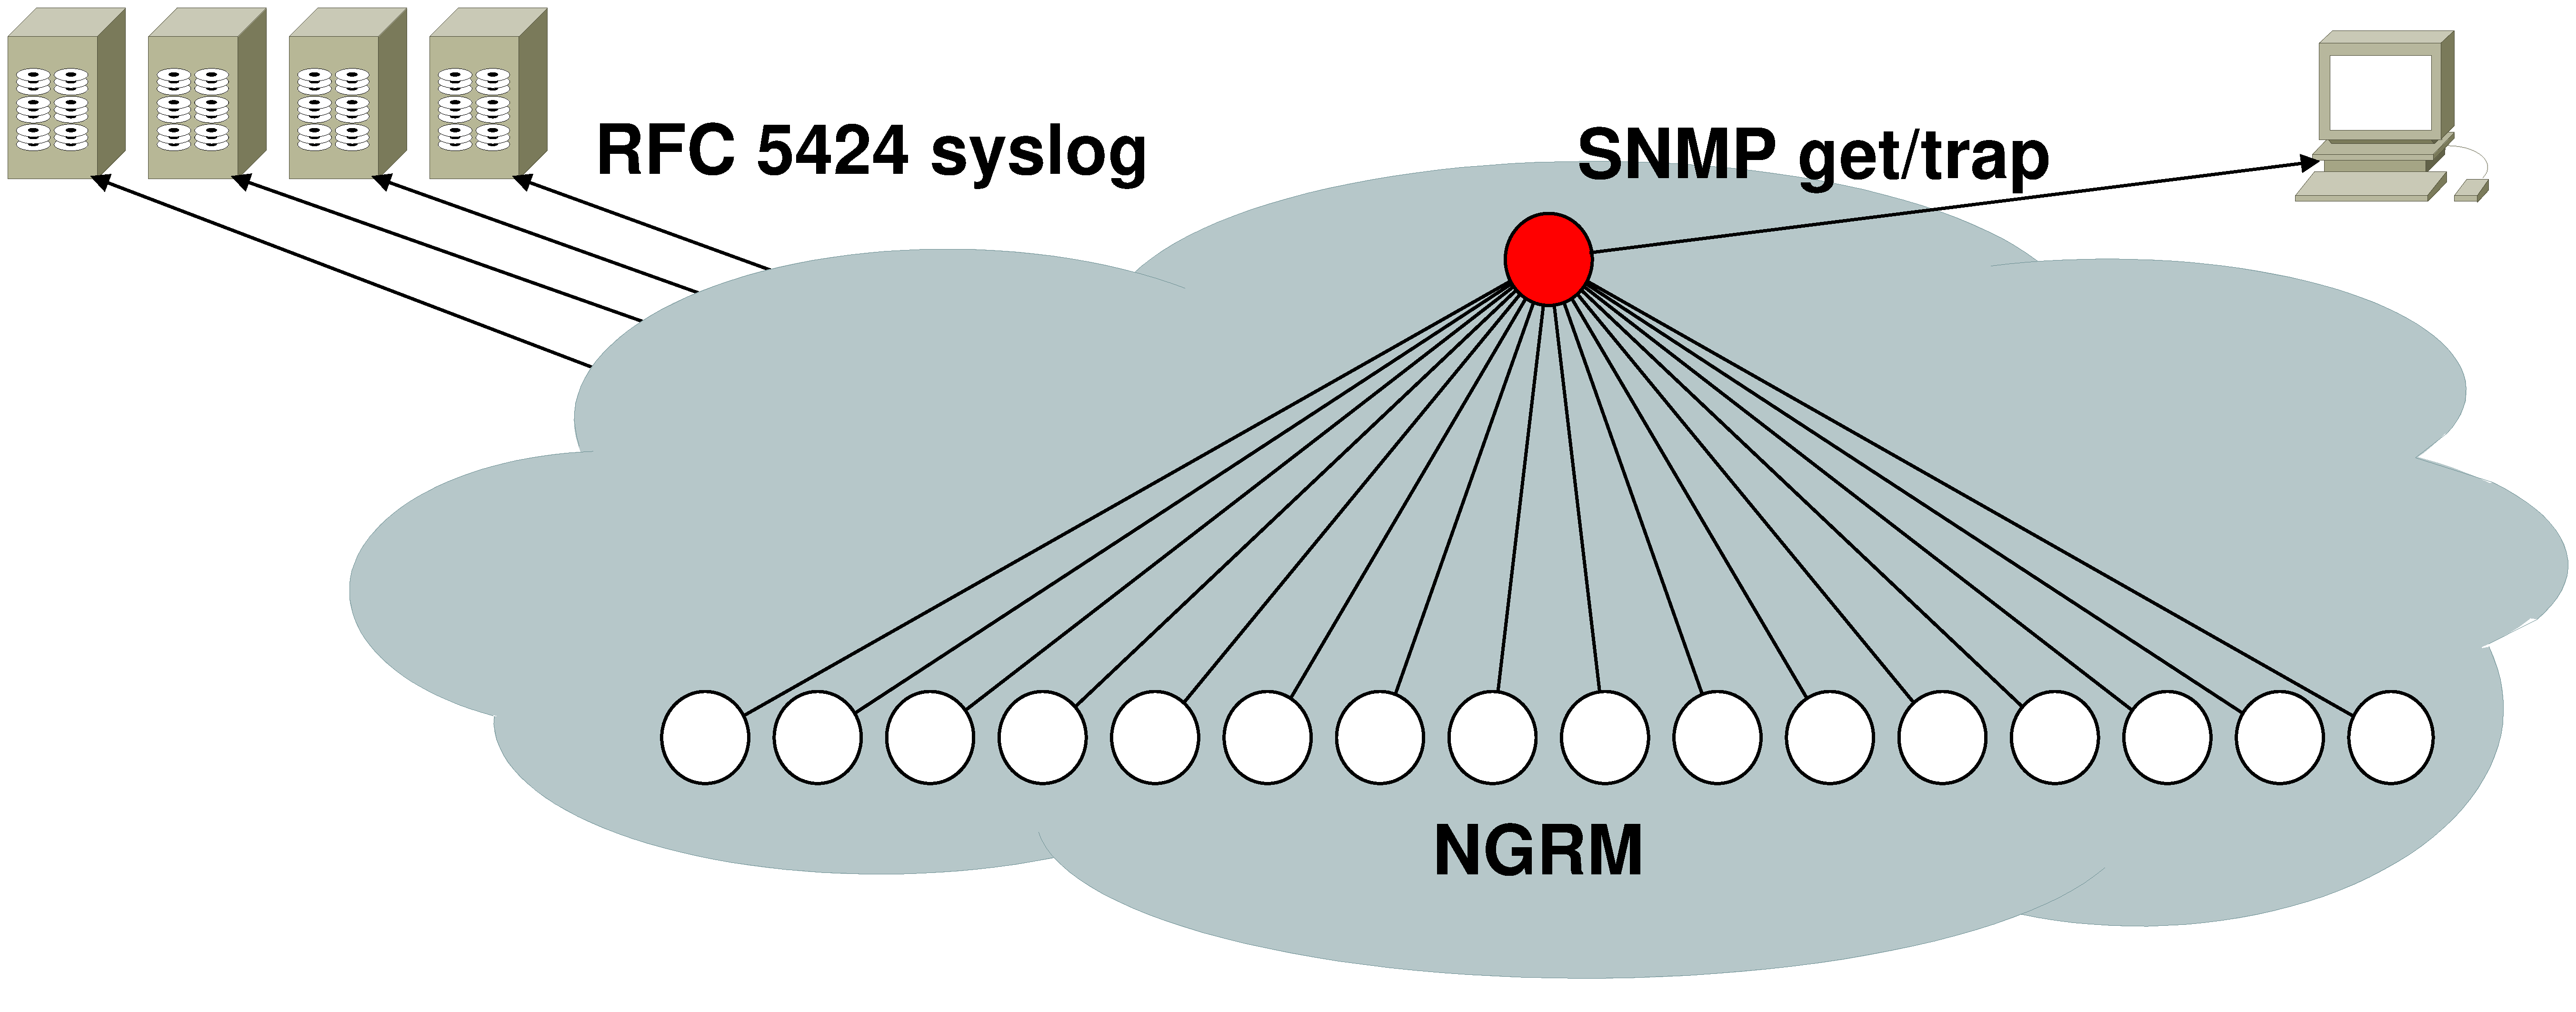
\includegraphics[scale=0.1]{../fig/mon_iface.eps}}
\caption{The \ngrm\ monitoring system interfaces with an external
enterprise monitoring system using SNMP, and with a persistent log
database using RFC 5424 structured syslog.}
\label{FigMonExt}
\end{figure}

The primary function of \ngrm's integrated monitoring is resource
health tracking.  This information is required in real time by schedulers
and runtimes to ensure that work is not launched on broken resources,
and that when things do go wrong, appropriate action can be taken.
In addition, \ngrm\ monitoring can be extended and customized
by sys admins and job owners to cover additional monitoring needs
that may be site, hardware, or job specific
(\ref{ReqsHiLevFun} req. 3.1).
Ideally \ngrm\ will be flexible enough to meet all
monitoring data aquisition requirements on compute nodes,
where our model is to synchronize monitoring interruptions within each job
and allow the system noise impact of monitoring to be tuned by the job owner
(\ref{ReqsHiLevFun} req. 3.0 and 3.2).

As shown in Figure~\ref{FigMonExt}, monitoring interfaces with an external
log database and enterprise monitoring system.
The log database is intended to be a comprehensive, schemaless, site-wide
store that will support a high insertion rate, large storage capacity,
and scalable queries.
As a record of all events in the data center, it will facilitate
postmortem analysis, enabling the correlation of job data with other
interesting occurrences that might not have been recorded in the job
database, or anticipated as something the job would normally ''care'' about.
Users will be permitted to inject application-level information into this
store and perform analysis with the system-level context there as well
(\ref{ReqsHiLevFun} req. 3.6).

The enterprise monitoring system is the mechanism used by operations center
staff and system administrators to monitor site systems which might include
\ngrm\ as well as facilities, network devices, storage appliances,
and non-\ngrm\ clusters.
This system is likely to already be in place at a site, thus common
protocols are chosen to reduce the effort required to integrate with \ngrm.

Monitoring state for a job is stored in the {\em resource database}, and
fault events are recorded in the {\em job database}.
These databases provide extensibility and persistence features described
in Section~\ref{sect:resdb} and \ref{sect:jobdb}.
Monitoring follows the \ngrm\ job recursion pattern, and is layered upon
the comms framework, which assigns each job a unique domain name within
the \ngrm\ private DNS namespace.
Live monitoring data can be obtained by using the resource
manager API to query the resource and job databases on the job's control
node, using the job's domain name.

Some applications and runtimes will require notification when system faults
occur.  For example, when a node that is part of a job crashes, or is about to
crash, some applications may be able to request a replacement node and recover.
To facilitate sharing of fault information, \ngrm\ will implement a
{\em fault notification service}.
Applications and runtimes use the fault notification service to produce
and consume fault events within the job.  In addition, a gateway on the
job control node allows software within the job to subscribe to faults
generated externally (such as by a file system used by the job), and to
publish certain faults that may be of interest to others.
Faults can change resource health state maintained in the resource database.
The {\em fault stream} produced by a job is logged in the job database
and can be considered part of the job's provenance record.

\ngrm\ Monitoring thus consists of
the plugin framework, 
log database interface,
fault notification system, and
enterprise monitoring interface.
Each of these parts is discussed below.

\subsection{Plugin Framework}

\begin{figure}
\begin{minipage}[b]{0.4\linewidth}
\fbox{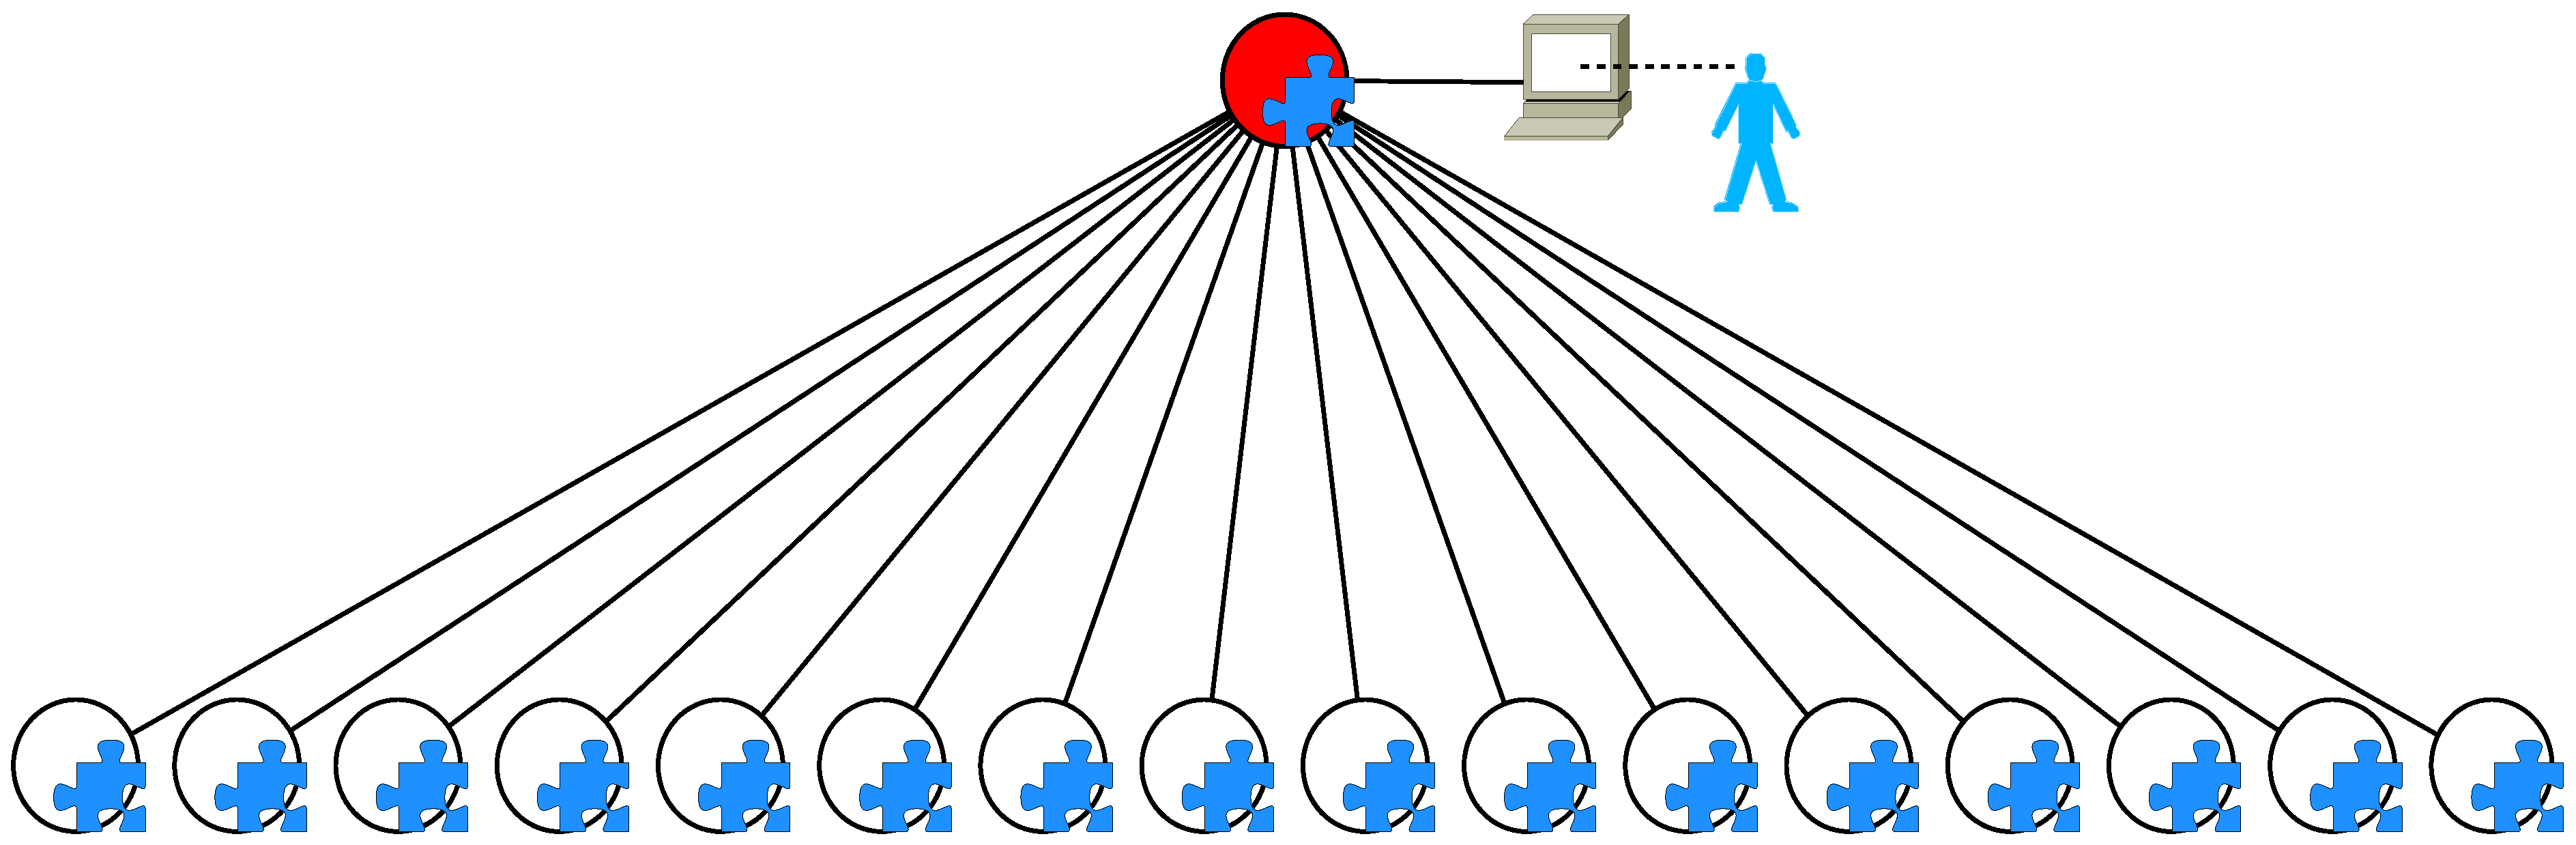
\includegraphics[scale=0.1]{../fig/mon_ex1a.eps}}
\end{minipage}
\hspace{1cm}
\begin{minipage}[b]{0.4\linewidth}
\fbox{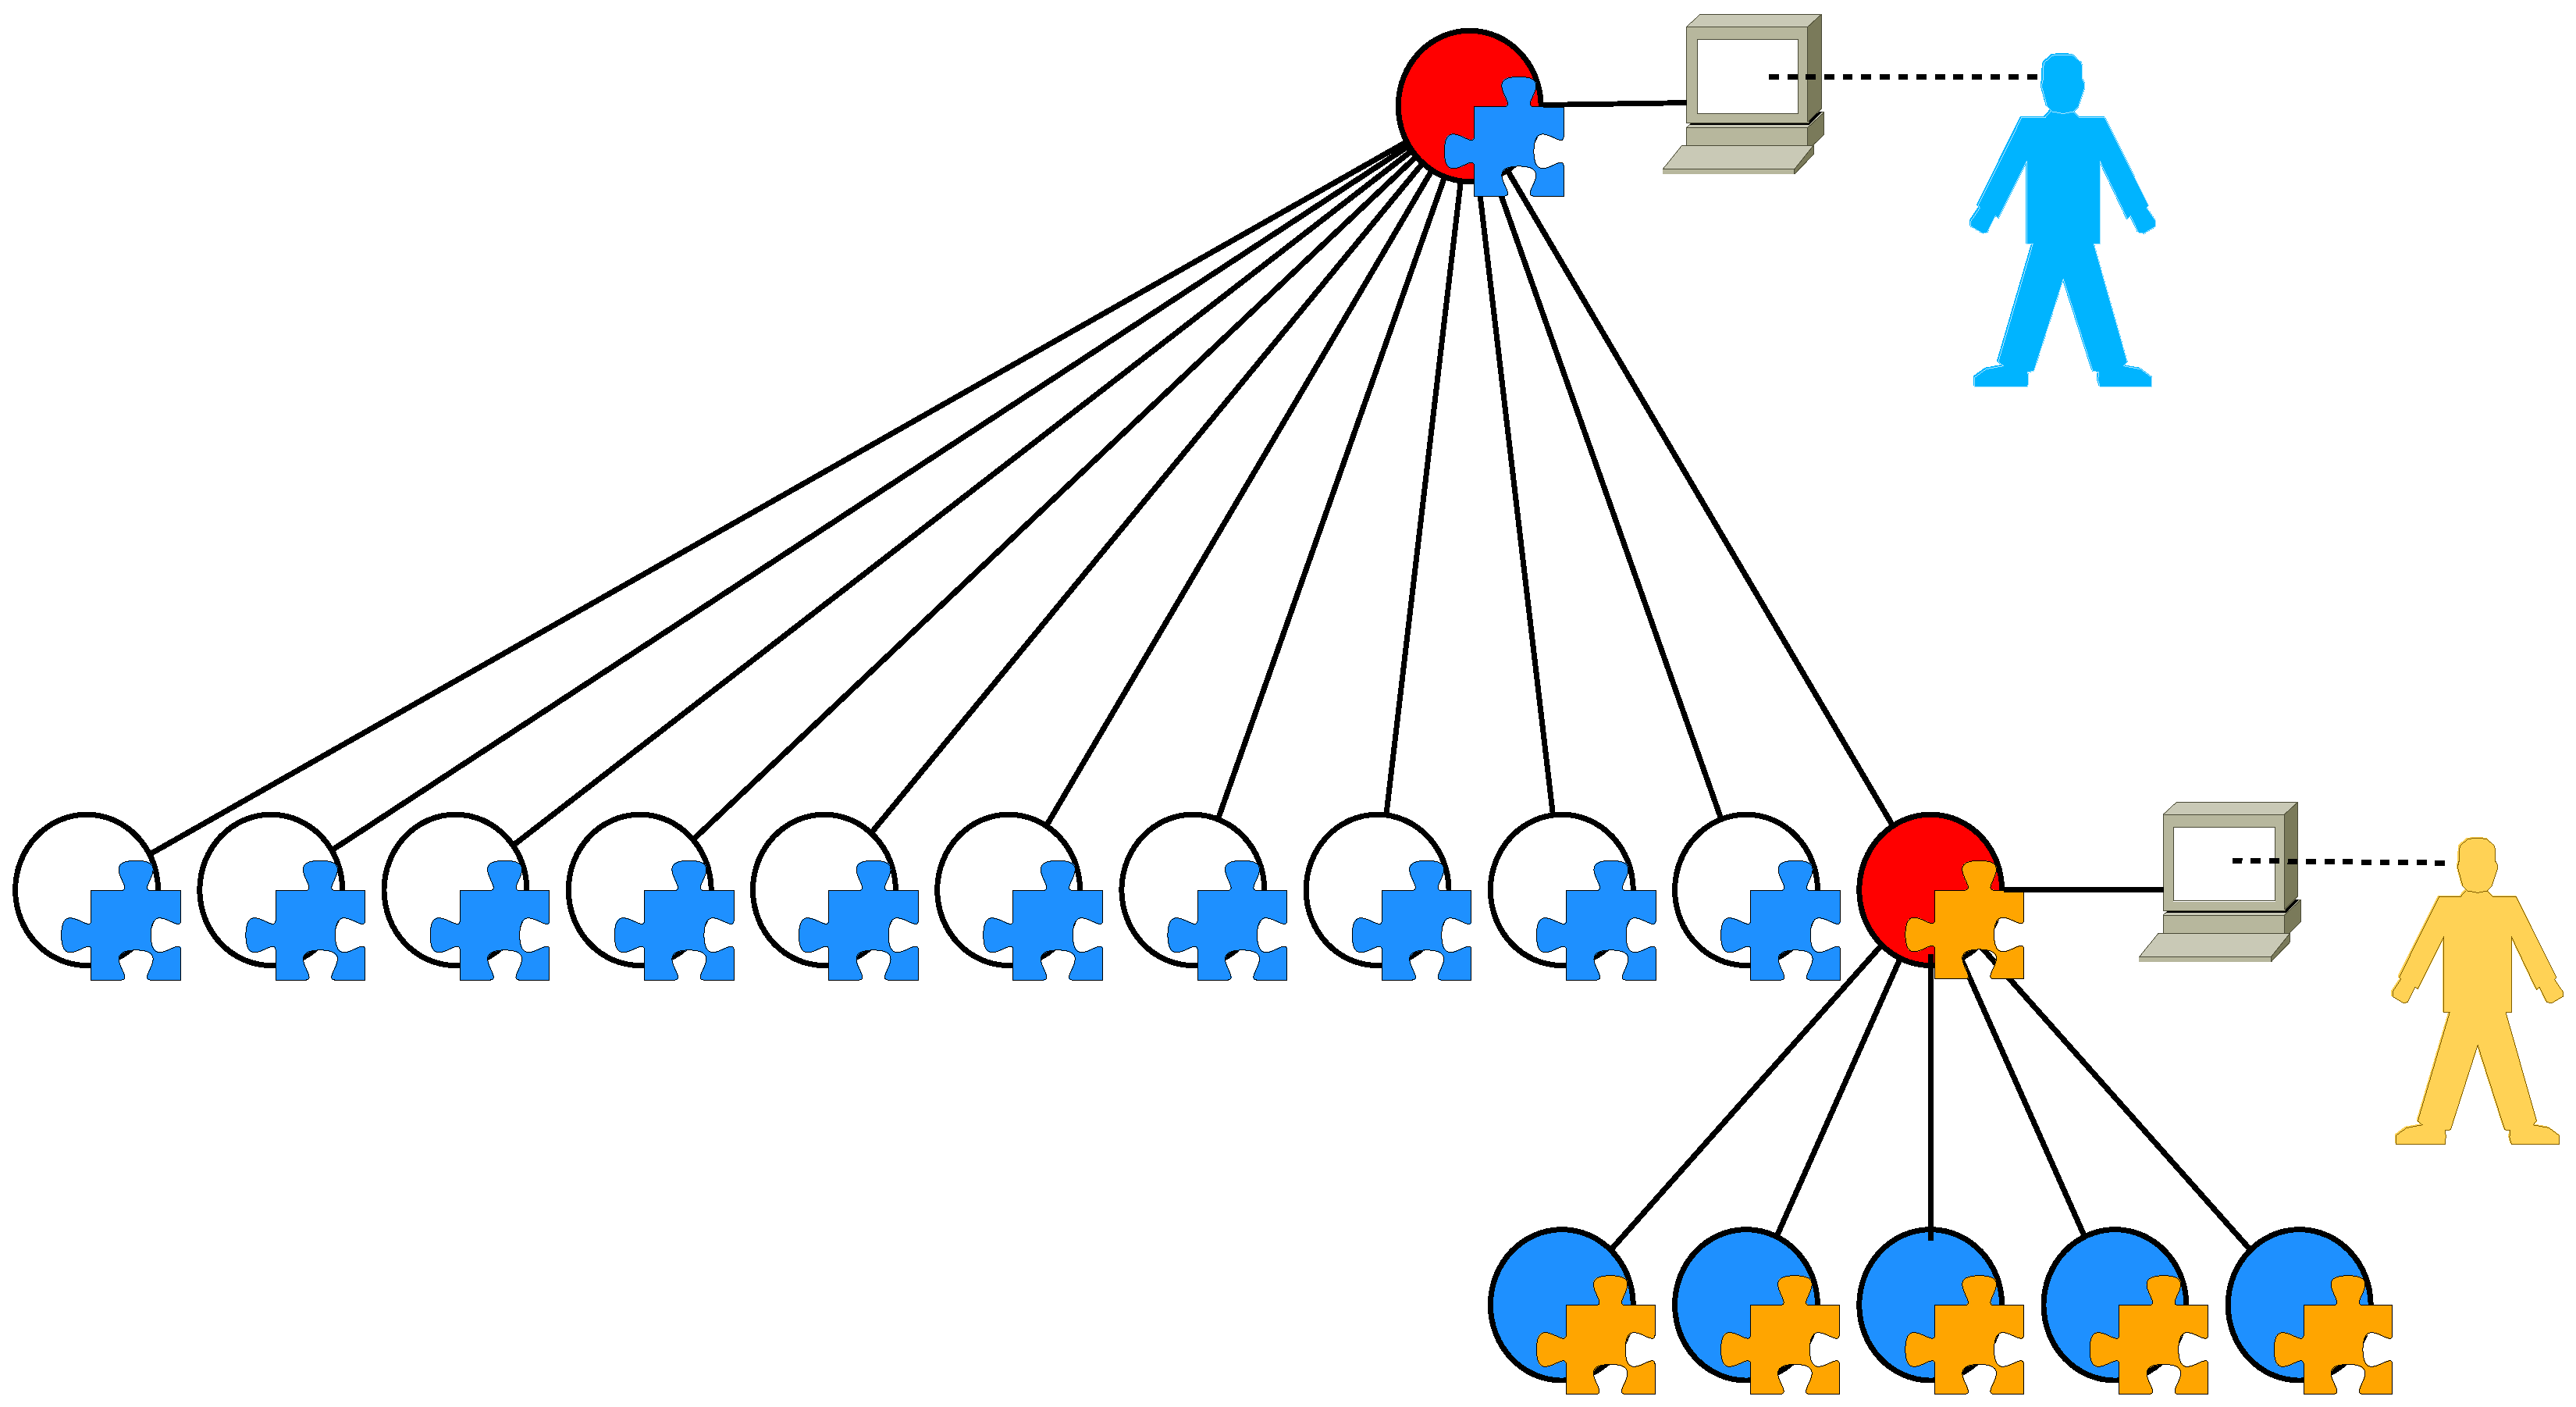
\includegraphics[scale=0.1]{../fig/mon_ex1b.eps}}
\end{minipage}
\caption{Monitoring follows the job hierarchy.
Control nodes (red) store resource status information in the resource
database and optionally export it via SNMP.
The monitoring plugin stack (jigsaw pieces) is customizable for each job.
Plugin execution is coordinated by the job's scheduling trigger event.}
\label{FigMonEx1}
\end{figure}

The monitoring plugin system provides a mechanism for arbitrary code 
contained in a user- or admin-provided plugin to be periodically
executed across a job.
The primary function of a plugin is to 
update resource health information in the resource database at the control node,
using the reduction network.
Plugins may also publish fault events and send data to the log database.
A default plugin stack is inherited by a job from its parent.
The set of active plugins as well as the trigger event period
which synchronizes execution can be tuned to a degree by the job owner.
The plugin framework is depicted in Figure~\ref{FigMonEx1}.

Plugins have three main functions: data source, data reduction,
and data sink.  Depending on the role of a node within the job or
its position on the reduction network,
one or more functions may be enabled on the node.
For example, a compute node may run only the data source function,
while the control node may run only the data reduction and data sink function.
Any function can publish fault events and send data to the log database
in addition to performing its role on the reduction network.

The data source function is driven by the scheduling trigger.
Its its purpose is to perform the first level of sampling or testing
of an object that is being monitored, and inject the resulting data 
into the reduction network.

The data reduction function accepts data coming from upstream source or
reduction functions of the same plugin.
Its purpose is to reduce the data in some way to improve scalability.
Reduced results are sent downstream, eventually to the plugin's sink function.
The execution of the data reduction function is driven by
incoming data and timers, not by the scheduling trigger.

The data sink function accepts reduced data from the same plugin on
the reduction network.
Its main purpose is to update resource state in the resource database,
although it could dispose of the plugin's data in other ways such as by
interfacing directly with a tool, or updating a database supplied by the
job owner.

Special care must be taken in the design of the plugin execution
environment to minimize disruptive impact on compute nodes.
For example, some monitoring systems like Chukwa\cite{Chukwa} require
data source functionality to execute in a Java VM, which would have an
unacceptably high memory and scheduling impact on some workloads.
Others like Nagios\cite{Nagios} rely on shell scripts that may have a
similarly high or unpredictable impact.
\ngrm\ monitoring plugins should leverage a lightweight execution environment
such as an embedded Lua\cite{LuaBook} interpreter.

\subsection{Log Database Interface}

Monitoring interfaces with an external log database intended to
be a comprehensive, schemaless, site-wide store that will support a
high insertion rate, large storage capacity, and scalable queries.
As a record of all events in the data center, it will facilitate
postmortem analysis, enabling the correlation of job data
with occurrences that were not actively tracked by the job during its
execution, thus not part of the canonical job record.

The log database, although implied by our requirements, 
(\ref{ReqsHiLevFun} req. 3.6), is ``outsourced'' by \ngrm\ with
a generic interface so that sites can choose the technology
to use to build such a system.  Some sites may prefer proprietary
systems such as Splunk\textsuperscript{\textregistered}, while others may
wish to build one from the many horizontally-scalable NoSQL databases
such as CouchDB\cite{CouchDB} or mongoDB\cite{MongoDB}.
Still others, operating at modest scale, may employ a traditional flat
file or relational database.  At LLNL, an in-progress Laboratory
Directed Research and Development feasibility study on HPC log
analytics\cite{LogLDRD} may spawn a separate project for the log database.

The syslog protocol, modernized in RFC 5424\cite{rfc5424},
includes a provision for STRUCTURED-DATA content,
an easily parsed format that is user-extensible.
Since log data may be voluminous at times, and scalability may require
a {\em distributed} log database implementation, it is not desirable to
use the \ngrm\ reduction network to funnel all log messages through the
single control at the root of the job.  Instead, we allow monitoring
plugin functions, or applications through the standard syslog
API\footnote{It is not clear that any available syslog API's handle
RFC 5424 STRUCTURED-DATA except as an opaque component of a textual
log message.  If one cannot be located, likely we will want to write
one to make management of structured data easier on users and ourselves.},
to inject data directly into an orthogonal syslog transport.
Syslog implementations already have standardized filtering, forwarding,
and security capability so there is no need to reimplement this within \ngrm.

To improve scalability in some situations, the reduction network can be
employed without necessarily resorting to control node funneling.
A monitoring plugin can log from the function (source, reduction, or sink)
that gives the right amount of reduction/funneling for the data managed
by that particular plugin.

\paragraph{Limiting unchecked log growth}
While it is well and good to design a capability for scalable, persistent
logging that is available both to system software and user applications,
growth of the log database should not be completely unbounded and unmanaged.
Two features could ease this problem: a {\em circular debug log buffer}, and
a {\em log insertion quota}.

Syslog verbosity is tunable by selecting the {\em level} of each
{\em facility} that is to be logged, from LOG\_EMERG (system is unusable)
to LOG\_DEBUG (debug-level message).  Usually system log levels are set
somewhere in the middle, but that means valuable log information leading
up to a failure is sometimes not available.  A solution to this problem is
to create a local circular debug buffer that logs at the maximum verbosity,
and tie the logging system into the job's fault notification service.
If a fault occurs in a particular facility, the circular buffer can be
dumped to the log database; otherwise the data is discarded as it is
overwritten.

Some log databases such as Splunk\textsuperscript{\textregistered},
have licensing based on ingest rates.  Such a system, or indeed other
systems that we wish to limit, could be operated with consumable resources
held by the resource manager.  For example, a job could request a certain
quota of log messages for the duration of its run.  When that number
is exhausted, a fault occurs.  This enables the \ngrm\ scheduler to ensure
that the ingest rate of the log database remains under control, while
giving users a new capability and a motivation to implement in-situ data
reduction.

\subsection{Fault Notification System}

The CIFTS group has argued\cite{CIFTS} that a wholistic, full-system approach
to fault notification is required in order to enable fault-tolerant
applications and runtimes to make good decisions when things go wrong.
For example, faults occuring on Lustre file system servers may be of interest
to a program controlling a suite of application runs, but traditionally,
file system failures are not reported in the application domain except
through system call failures.
\ngrm\ addresses this need with a fault notification system based on
the comms layer's reduction network and PUB-SUB event notification service.
Fault notifications are published (by monitoring plugins, applications, etc)
to subscribers within the job.
A {\em fault gateway} allows configured local faults to be published externally,
and configured external faults to be published locally.

We have adopted the 
CIFTS Fault Tolerance Backplane API\cite{FTBAPI} (FTB-API)
an emerging standard for fault notification available in some MPI
implementations and other software as the programming interface for the
fault system.  We will use CIFTS event namespace conventions as well.
This choice reduces the overhead of porting fault-tolerant runtimes and
other software between systems, and allows FTB-API based implementations
to be immediately functional on \ngrm.

While the CIFTS reference implementation defines a {\em backplane}
architecture for fault notification, our fault notification system
leverages both the hierarchical relationship between jobs (local vs global
fault scope), and the reduction network within a job (reducing duplicate
or same-root-cause faults) to achieve greater scalability and more intelligent
fault processing.
Faults can be directly published across the job via the comms event
notification service, but when data reduction is desirable, monitoring 
plugins can be employed to route faults through a reduction sieve to
the control node where they are published in processed form.
Monitoring plugins are also employed when the occurence of a fault needs
to affect resource health state in the resource database.

The fault gateway, running on the job's control node, 
integrates the job's fault notification domain with the system's.
It re-publishes a configurable set of local faults to the parent job, 
which forwards them to its parent, and so on, reaching subscribers anywhere
in the system.
Conversely, the fault gateway subscribes to a configurable set of global
faults in the parent job and re-publishes them locally.
In this way, external faults "of interest" to any job become part of the
job's local fault domain.

The job's {\em fault stream} thus becomes an important record of anomolous
conditions occuring within the job and those of interest occuring outside
the job.  It is stored in the job database.

\subsection{Enterprise Monitoring Interface}

Site operations centers and system administrators use
monitoring to track problems that may require someone's intervention, and
to gain insight into how the systems they are responsible for are being used.
The systems that are monitored may include clusters as well as facilities
and networking equipment.
\ngrm\ monitoring gathers resource health information that is an important
component of that view, and indeed aims to replace other compute node
resident monitoring frameworks in an effort to synchronize monitoring
interruptions across jobs.
Although \ngrm\ will provide tools for viewing its internal operation
including resource health, it must also export resource health information
to external enterprise monitoring software to allow \ngrm\ to be integrated
into a site-wide monintoring strategy, perhaps already deployed.
We accomplish this using our hierarchical job model to ensure that
{\em actionable} fault information is available in the root job resource
database, and develop a gateway to export this information
to external enterprise monitoring software.

The health state of resources is maintained in the resource database of
each job.
This state is initialized from the parent resource database at job inception
and is transferred back to the parent at job teardown.
In addition, some fault events within a child job are published
to the parent and thus may alter resource state in both the parent and
the child (perhaps driven by the need for enterprise monitoring to see them).
Therefore, although each job is given a delegation to monitor the resources
allocated to it, resource health state does, with varying degrees of latency,
eventually recurse to the root job's resource database, thus it is
appropriate to interface enterprise monitoring there.

SNMP\cite{StallingsSNMP} is the de-facto standard protocol for enterprise
monitoring.  An SNMP gateway that speaks both the resource database API
and SNMP will run on the root job's control node.
State can be {\em pulled} out of \ngrm\ via SNMP GET and GETBULK requests.
After an initial state transfer, state changes can be {\em pushed}
by \ngrm\ via SNMP TRAP requests.  This model supports multiple external
management entities.
Theoretically the SNMP gateway could run on any job, if desired.
For example, long running service entities like Lustre server clusters
could be ''peeled off'' of the root instance, assigned to a child job,
and monitored separately.
Practically speaking, jobs configured for external monitoring should be
long lived.

A base set of \ngrm\ management data will be defined in an \ngrm\ 
enterprise-specific management information base (MIB) module.
The set of data exported by the SNMP gatway can be extended by adding
new MIBs that map new SNMP objects to resource database objects.
%FIXME: can we use the Resource Description Language (RDL) to simplify
%the creation of custom MIBs?

\ifwbs
\subsection{Monitoring WBS}

\begin{longtable}{|p{1cm}|p{10.2cm}|p{1cm}|p{1cm}|p{1.8cm}|}\hline
  \textbf{Item} & \textbf{Description}
                & \textbf{Deliv}\footnote{SD = software drop,
                        DR = design review, V = viewgraphs, D = document}
                & \textbf{Weeks} & \textbf{Depend} \\
  \hline
  \hline
  \multicolumn{5}{|l|}{3.3. \textbf{Monitoring Plugin System}} \\
  \hline
  3.3.1.& Design/prototype plugin system including structured log format
	  and event naming.  (See also possible CIFTS/FTB tie-in in runtime).
          (See also Meyer monitoring project).
	& DR
	&
	& comms \\
  \hline
  3.3.2.& Implement plugin system.
        & SD
        &
        & 3.3.1 \\
  \hline
  3.3.3.& Document process for creating monitoring plugins.
        & D
        &
        & 3.3.1 \\
  \hline
  3.3.4.& Design/prototype a set of default plugins including plugins
          for instrumenting jobs to gather "implicit provenance" such as
          file accesses.
        & DR
        & 
        & 3.3.1 \\
  \hline
  3.3.5 & Implement set of default plugins.
        & SD
        &
        & 3.3.4 \\

  \hline
  \multicolumn{5}{|l|}{3.4. \textbf{Monitoring Console}} \\
  \hline

  3.4.1.& Design/prototype HTTP/REST monitoring console.
          (Long/Martinez Lorenz team)
          (See also Meyer monitoring project).
	& DR
	&
	& 3.3.1 \\
  \hline
  3.4.2.& Implement monitoring console.
	& SD
	&
	& 3.3.1, 3.4.1 \\
  \hline
  3.4.3.& Design/prototype Lorenz integration.
	  Think about how monitoring console integrates with the myllnl
	  dashboard experience.
          (Long/Martinez Lorenz team)
	& DR
	&
	& 3.4.1 \\
  \hline
  3.4.4.& Design/prototype skummee integration.
          How will \ngrm\ integrate with ops monitoring view?
          How will out of band monitoring (IPMI, DDN's, etc) integrate with
	  monitoring console?
          (Meyer monitoring project).
	& DR
	&
	& 3.4.1 \\
  \hline
  3.4.5.& Implement Lorenz/skummee integration.
	& SD
	&
	& 3.4.3, 3.4.4 \\
  \hline
  \multicolumn{5}{|l|}{3.5. \textbf{Monitoring Database Interface}} \\
  \hline
  3.5.1.& Study available NoSQL databases for 100K node scalability
          and appropriate query interface.
          Use offline log data to investigate system diagnostic capability
          and prototype queries.
          (Gamblin/Mohror HPC Data Analytics FY12 LDRD)
        & V
        & 
        & LDRD \\
  \hline
  3.5.2.& Implement prototype database tied to live log sources.
          Study scalability and develop queries.
          (Gamblin/Mohror HPC Data Analytics FY12 LDRD)
          (See also: Faaland SPLUNK deployment).
        & DR
        & 
        & 3.5.1 \\
  \hline
  3.5.3.& Design/prototype access-role based security.
        & DR
        & 
        & 3.5.2 \\
  \hline
  3.5.4.& Design/prototype schemas and queries for reporting
          RAS metrics of interest to center management.
        & DR
        & 
        & 3.5.2 \\
  \hline
  3.5.5.& Design/prototype procedure for sanitizing and releasing data
	  for research study and citation.
        & DR
        & 
        & 3.5.2 \\
  \hline
  3.5.6.& Design/prototype schema for job logs and queries for
          associating job data, system log data, etc..
        & DR
        & 
        & RM, 3.5.2 \\
  \hline
  3.5.7.& Implement database.
        & SD
        & 
        & 3.5.2, 3.5.3, 3.5.4, 3.5.5, 3.5.6 \\
  \hline
\end{longtable}
\fi

